\section{The Future of Information Retrieval}

It's easy to be impressed with how capable modern search engines are compared to what we had in the 1950s, as it is easy to be impressed by how much smarter a frog is compared to a hat. While search engines can do some really really really good stuff, IR research has many obstacles on it's long road ahead. A feature search engines could one day possess, is provided by Douglas Hofstadter below.

% \vspace{\baselineskip}
\begin{quote}
``search engines can instantly search billions of Web sites for passages containing the phrase `in good faith', yet are incapable of spotting Web sites in which the idea of good faith (as opposed to the string of alphanumeric characters) is the central theme?''
    \begin{flushright}
        --- Douglas Hofstadter, Surfaces and Essences
    \end{flushright}
\end{quote}

Identifying a \textit{central theme} in a text would be powerful, one could perform \textit{intertextual} analysis. Regardless of what the future might hold it is clear IR research will outgrow text based retrieval. Which is what we have started to see, over the past few years IR research has started the shift from language-oriented systems towards of cognitive-oriented systems. We have already started seeing systems that transcend term matching, and their results are promising. For example, GPT-3 (Generative Pre-trained Transformer 3) is a language model (LM) that already outperforms non-experts on text comprehension and text understanding \cite{wang2019superglue}, like The Stanford Question Answering Dataset \cite{rajpurkar-etal-2016-squad}. GPT-3 was released in June 2020, and since that date, we have seen a Cambrian explosion of research into Natural Language Understanding (NLU). The most effective NLU systems (e.g.\ GPT-3, BERT, OpenAI) all use deep learning approaches.














% and find books which are similar in theme, concept, structure, subject material, etc. One could (hypothetically) find the literary inspiration for James Joyce's Ulysses in Homer's Odyssey. Or the Christ Narrative in the Narnia Series. Or Shakespeare's Hamlet in The Lion King. Or Shakespeare's Romeo and Juliet in West Side Story. Or Shakespeare's Hamlet in Akira Kurosawa's Throne of Blood. Or Shakespeare's Romeo and Juliet in Gnomeo \& Juliet. Basically any good movie, play, and book has taken inspiration from Shakespeare.

% Shakespeare himself was even inspired by other authors (namely Greek writers). The following example from Mark Forsyth \cite{forsyth2014elements} proves beyond doubt that Shakespeare did indeed plagiarize text (without attribution). He used his poetic license to reorder words, substitute synonyms, add details, creating alliteration, scansion, and other figures of rhetoric.

% \newpage

% \noindent
% Here is an excerpt from Shakespeare's Antony and Cleopatra, Act II Scene II.
% \begin{quote}
%     ``The \hlcyan{barge} she sat in like a burnished throne, \\
%     Burned on the water: \hl{the poop was beaten gold};\\
%     \hlgreen{Purple the sails and} so perfumed that\\
%     The winds were lovesick with them; \hlpink{the oars were silver,\\
%     Which} to \hltwo{the tune of flutes} \hlone{kept stroke}, and made\\
%     The water which they beat to follow faster,\\
%     As amorous of their strokes.''
%     \begin{flushright}
%         --- Shakespeare, Antony and Cleopatra, 1607 AD
%     \end{flushright}
% \end{quote}

% \noindent
% And here's an excerpt from a biography of Cleopatra written, 1,400 years earlier.

% \begin{quote}
% ``...to take her \hlcyan{barge} in the river Cydnus,
% \hl{the poop whereof was of gold}, \hlgreen{the sails of purple, and}
% \hlpink{the oars of silver, which} \hlone{kept stroke} in rowing
% after the sound of \hltwo{the music of flutes}''
%     \begin{flushright}
%         --- Plutarch, Parallel Lives, 2nd century AD
%     \end{flushright}
% \end{quote}

% Shakespeare wasn't a supernaturally gifted genius. He was a well-read hard-working writer. He studied Greek language and Greek rhetoric, then applied that knowledge to English. Using what he learned, he executed scripts and characters with sharp wit and axes.

% This level of intertextual analysis requires an expert on Shakespeare, and an expert on Roman history, and coincidence to find the similarity between these documents.  

% \footnote{My first ever double zeugma! \textit{``To kill the boys with the luggage!''} is a zeugma Shakespeare wrote in Henry V and iambic pentameter.}.


% Or possibly find the similarities between movies
% You could find the similarities between Bridget Jones's Diary and Pride and Prejudice.  
% King Kong as an allegory for the African slave trade.
% , and 
% Throne of Blood Hamlet
% West Side Story
% Snowpiercer has many parallels to Willy Wonka \& the Chocolate Factory
% The Jesus Narrative in Narnia, Star Wars, Harry Potter, the Matrix, Buffy the Vampire Slayer, 
% various episodes of The Simpsons are parodies of many 




% \begin{figure}[!b]
%   \begin{subfigure}[b]{0.49\textwidth}
%     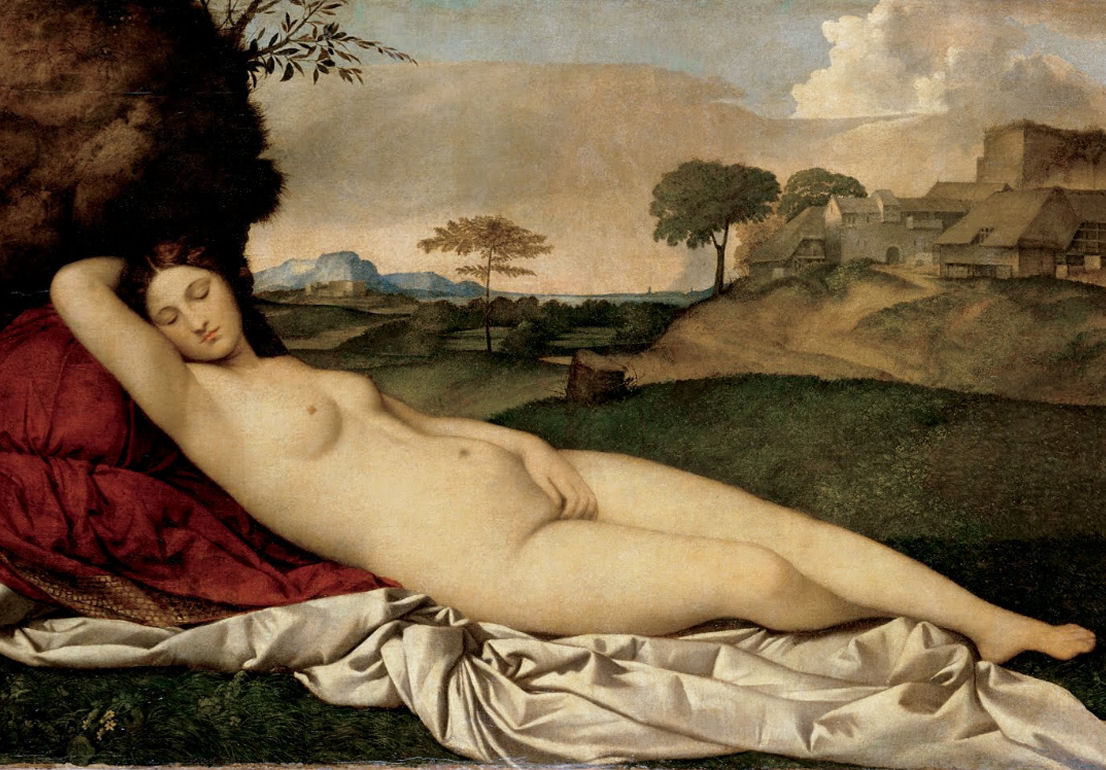
\includegraphics[width=\textwidth]{graphics/Sleeping Venus Giorgione1508-1510.jpg}
%     \caption{Georgione's Dresden Venus 1508-1510}
%     % \label{fig:cave}
%   \end{subfigure}
%   \hfill
%   \begin{subfigure}[b]{0.49\textwidth}
%     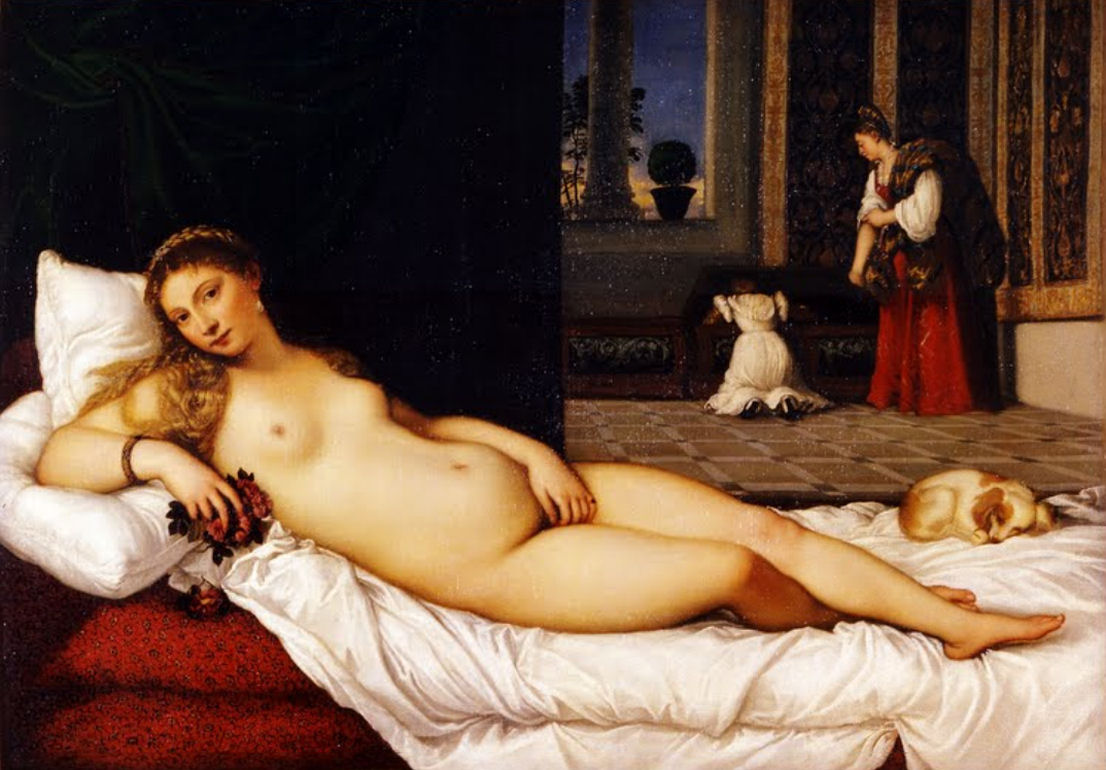
\includegraphics[width=\textwidth]{graphics/Venus of Urbino Titan 1538.jpg}
%     \caption{Titan's Venus of Urbino, 1538}
%     % \label{fig:picasso}
%   \end{subfigure}
%   \caption{Standard image retrieval methods fail to match these paintings as there is substantial difference in appearance.}
%   \label{fig:paintings}
% \end{figure}

% The Dresden Venus by Giorgione (1510)

% Venus of Urbino by Titian (1538)

% If we could build a system that could see the conceptual structure and theme of a text, we could 





% I think Information \textit{Retrieval} will be superseded with Information \textit{Generation} and procedural creativity. Having a machine with \textit{creative} capabilities does not mean they will supersede artists, as computer graphics did not supersede animators. Computers are already tools that artists use, developing computational creativity would just be another tool to use. 

% There are currently many skeptics, who deny that machine can be truly \textit{``creative''}. Inspiration was once thought to be a blessing from the divine.

% \begin{flushleft}
% ``Sing to me Muse...''
% 	\\--- Homer
% \end{flushleft}
% \begin{center}
% ``For the Lord giveth wisdom''
% 	\\--- Proverbs 2:6
% \end{center}
% \begin{flushright}
% ``that Divine accident from the gods, from the mysterious source of the inexplicable''
% 	\\--- Søren Kierkegaard
% \end{flushright}

% In human history, unexplained phenomena are usually credited to divine intervention; eventually, science catches up and gives it a qualifying explanation. Something which cannot be explained feels like magic. The moment you understand an explanation, it transforms into a mere trick. Some prefer not to kill the magic, not look behind the Wizard’s curtain, not explain a joke. But, reverse engineering a construction or a process is the first step in being able to to reproduce it yourself, simulate its external behaviour, or emulate its internal properties.

% However, long before the technological singularity arrives, we will probably get our hands on some super cool search engines.



% \section{Conceptual Semantics}
% Text was replaced with knowledge. The popularity of knowledge graphs as a data structure rose. These graph based, knowledge representations were thought to be a rough approximation of the knowledge structures within our mind. The dream was to build knowledge systems on a massive scale, these highly structured and content-rich ontologies, which we could traverse to find any piece of information, and develop algorithms which could traverse the ontologies for us. A big issue with these systems is that they're expensive to build and maintain, they're essentially infeasible in practice.

% The next ambitious goal for IR research is Conceptual Semantics. A proposed symbol system intended to resemble our thoughts better than language does. If we had an algorithm that could perform \textit{perfect} semantic disambiguation and determine the author's original intent. One could index documents as \textit{conceptual symbols}, not lexical terms. Search queries could also be converted concepts. And performing a search task would involve matching concepts directly. These kinds of systems would not require the effort to manually build or maintain. Such a system could indeed transcend language barriers.

% https://mydailyartdisplay.wordpress.com/2011/02/15/venus-of-urbino-by-titian-and-the-sleeping-dresden-venus-by-giorgione/






% Having a knowledge structure, or ontology, with clearly defined boundaries, and consistent category membership. Is only really ideal building human interfaces. Expecting a person to find a single book from a pile of millions would be infeasible in practice, but shelve those books under filing system, or index, it becomes feasible. Imposing handmade structure onto large volumes of information makes it possible for to navigate, explore, and find what we're looking for. But it appears that handmade, orderly structure is not what makes for  




% language was thought to mirror our cognition
% though it has become increasingly apparent that this is not the case
% language and cognition are related
% but our understanding is when the speaker's intent and the listener's inference agree


%%%%%%%%%%%%%%%%%%%%%%%%%%%%%%%%%%%%%%%%%%%%%%%%%%%%%%%%%%%%%%%%%%%%%%%%%%%%%%%%%%%%
% \section{}


% It should be clear that language is highly ambiguous, but surprisingly our thoughts do not seem to be. At least the thoughts of a healthy, neuro-typical mind are not ambiguous. However, the mind of someone suffering from schizophrenia can have great troubles disambiguating their own thoughts \cite{torrey1985surviving}.

% \begin{center}

% \textit{``Simple words such as `eye' can be substituted for `I' and `to' for `too' or `two'. Homonyms have significant meaning to the schizophrenic, as you can see, or should I say sea. Words like no and know can be used interchangeably. So when I answer a question `no' I may very well be simply asking the question `know?' As in `do you know?' ''}
% \\ --- Surviving Schizophrenia, 6th Edition: A Family Manual
% \end{center}


%%%%%%%%%%%%%%%%%%%%%%%%%%%%%%%%%%%%%%%%%%%%%%%%%%%%%%%%%%%%%%%%%%%%%%%%%%%%%%%%%%%%